% The verified statement, read exactly -- drafted by loop0015 item 02 (2026-11-05),
% rewritten in plain English by item 08x (2026-11-05, owner's rule of 05:30).
% Every line number of the comparator file is at commit 4eaee875 of the clone
% (~/dev/untrusted/openai-math, read with cat/sed -n only); every manuscript quote
% gives the page of paper.pdf and the line of reports/scratch/eth_audit/paper.txt.
% Every number of this section: python3 -I paper3/scripts/runtime_scale.py
% (the rho(n)/n table and the crossings) and python3 -I
% reports/scratch/eth_audit/check_encoding.py (the encoding lengths).
% The definition-by-definition reading and the theorem with its quantifiers
% are in Appendix B (secB_appendix_technical.tex), cited from here.
\section{The verified statement, read exactly}
\label{sec:statement}
\begingroup\sloppy

\subsection{What we are reading, and the words we need}
\label{sec:statement-words}

OpenAI's collection \citep{OAI:The-Exponential-Time-Hypothesis-is-False-October-25-2026}
holds, for the result it calls family 378, one machine-checked theorem.
It is named \path{exact_count_and_sat}. It is stated in the family's
challenge file, which is 220 lines long:
\clonefile{lean/ComparatorChallenges/SubexponentialSAT.lean} at commit
\texttt{4eaee875} of the collection. This section reads that
file and says what the theorem asserts and what it does not. Line
numbers are those of the file. We quote nothing from memory.

A few words first, each in one sentence.
\emph{Lean} is a proof assistant: a program that checks every step of a
proof and refuses a proof with a gap.
The \emph{kernel} is the small core of Lean that does the final
checking; when we say a statement is verified, we mean the kernel
accepted a proof of it.
A \emph{formula} here is a Boolean formula in conjunctive normal form: a
list of \emph{clauses}, each clause an ``or'' of a few variables or
negated variables, and the whole formula true when every clause is
true. A \emph{$k$-CNF} is such a formula whose clauses have at most $k$
variables each; 3-SAT is the problem of deciding whether a 3-CNF can be
made true.
A \emph{satisfying assignment} is a choice of true or false for every
variable that makes the formula true; with $n$ variables there are
$2^n$ assignments to try, and \emph{trying all $2^n$ assignments} is the
method the title names.
The \emph{comparator} is OpenAI's checking tool. It takes a
\emph{challenge file}, which states a theorem and leaves the proof blank,
and a \emph{solution}, which proves it, and checks that the two state
the same theorem and that the proof uses only three standard axioms. An axiom is a statement accepted without proof; the three standard ones are the ones every ordinary mathematical proof in Lean uses.
The file we read is the challenge file. It carries the statement with
the placeholder \texttt{sorry} where the proof would go (line 218). The
solution proves the same statement in 3,091 files
(Section~\ref{sec:proof}). We rebuilt that proof ourselves and the
kernel reported the three standard axioms and nothing else
(Section~\ref{sec:replay}).

\subsection{The definitions, in words}
\label{sec:statement-definitions}

The theorem speaks about five kinds of object. Each is defined in the
file before the theorem. Appendix~\ref{app:tech-definitions} gives
every definition with its line numbers; here is what each one means.

\paragraph{Formulas and the count (lines 13--51).}
A formula is a finite set of clauses over $n$ variables, and a clause is
a finite set of signed variables. The formula \texttt{F} has width at
most $k$ when every clause has at most $k$ members (line 38). The number
\texttt{count F} is how many of the $2^n$ assignments make the formula
true (line 47). Because clauses and formulas are sets, a repeated clause
collapses into one; the empty clause is allowed and can never be
satisfied; and a clause holding both a variable and its negation is
allowed and counts as two members. The manuscript says the same thing in
its own words: ``Repeating a literal permits clauses with fewer than
\(k\) literals'' (p.~1, lines~44--45).

\paragraph{The input encoding (lines 53--81).}
The machine does not read a formula; it reads a string of bits. The
file fixes how a formula becomes bits. Numbers are written in unary,
that is, $n$ is written as $n$ ones and a zero. Each clause becomes a
sorted list of such numbers, the formula becomes a list of clauses, and
the number of variables is written in front. Two things matter. First,
the number of variables is part of the input, so a variable used in no
clause still counts. Second, the string is not long: its length is a polynomial in $n$ and $m$, which means it grows like a fixed power of them and not like $2^n$. A formula with $m$ clauses of width $k$ on $n$ variables takes at most about $8\,k\,n\,m$ bits. In symbols, with $L$ the length of the string,
\[
  L \;\le\; n + 2 + m\,\bigl(2k(4n+1) + 4\bigr) \;=\; O(k\,n\,m),
\]
where $O(k\,n\,m)$ is read ``at most a fixed multiple of $k\,n\,m$''.
One random formula with 125 variables, 500 clauses and width 4 becomes
$1{,}006{,}223$ bits; one with 1,000 variables, 4,000 clauses and width
3 becomes 47.9 million bits. Both numbers are from a script that
imitates the definitions on formulas it draws with its random seed fixed
at 1, \repofile{reports/scratch/eth_audit/check_encoding.py}; the length
depends on which literals a formula holds, so another formula of the same
size gives a nearby number, always under the bound. Nothing in the
encoding grows exponentially.

\paragraph{The machine (lines 83--128).}
The machine is a Turing machine, the textbook model of a computer: a finite control that reads and writes symbols on tapes, one cell at a time. This one has several tapes: a finite table of states, a finite number of tapes, and a rule that, in each state, reads
one cell of one tape and then either stops with a yes-or-no answer, or
writes one symbol, or moves one head by one cell. Every part of it is
finite. A step is one lookup in a table with three rows per state. No
part of the machine can hide an unbounded computation inside a step.
The tapes and the moves are Mathlib's standard ones (Mathlib is the
community library of mathematics for Lean, at the revision the
collection pins, \texttt{d13f23b7}).

\paragraph{Runs (lines 87--90).}
A \emph{configuration} is a snapshot: the control's current state and the contents of every tape. A \emph{trace} of length $t$ is a record that the machine, started in one configuration, reached another in exactly $t$ successful steps. The
step rule is a function, so each run is determined by its input; there
is no randomness and no guessing.

\paragraph{Space monitoring (lines 147--189).}
Beside each configuration the file keeps, for every tape, the furthest
cells the head has reached to the left and to the right. The
\emph{visited space} is the total number of cells ever visited, summed
over the tapes. The \emph{count word} is a number written in binary,
least significant bit first (line 147).

\paragraph{The exponent and the bound (lines 130--141).}
The theorem's running-time bound is built from one function of $n$,
which the file calls \texttt{runtimeScale} and we write $\rhon$:
\[
  \rhon \;=\; \frac{n\,\bigl(\ln\ln(n+16)\bigr)^2}{\sqrt{\ln(n+16)}},
\]
with $\ln$ the natural logarithm. In words: take $n$; multiply it by
the square of the logarithm of the logarithm of $n + 16$; divide by the
square root of the logarithm of $n + 16$. The manuscript uses the same
logarithm: ``Throughout, log denotes the natural logarithm'' (p.~1,
lines 48--49; again at p.~7, lines 326--327). The $+16$ keeps the double
logarithm defined and positive at every $n$, including $n = 0$, so the
theorem needs no condition on $n$. The bound itself, called
\texttt{runtimeBound} (lines 136--139), is
\[
  C\,(L+1)^d\,2^{A\,\rhon},
\]
that is, a constant $C$, times a power $d$ of the input length $L$,
times two raised to $A$ times $\rhon$. We call $\rhon$ \emph{the
exponent} and $C(L+1)^d\,2^{A\rhon}$ \emph{the bound} throughout the
paper. The constants $C$, $A$ and $d$ are the subject of the next
subsection.

\subsection{What the theorem says, and in what order}
\label{sec:statement-theorem}

Lines 194--217 state the theorem. Appendix~\ref{app:tech-theorem}
displays it with every quantifier and the line of every clause. In
words, for every fixed width $k$ of at least 2:

\begin{quote}
There exist a machine, a count tape, an answer tape, and five positive
constants $C, A, S, d, e$, such that for every number of variables $n$
and every formula $F$ on $n$ variables of width at most $k$, the
machine started on the encoding of $F$ halts after some number of steps,
\texttt{time}, with the count of satisfying assignments written in
binary on the count tape, the bit ``is the count positive'' on the
answer tape and in its halting state, a count word of at most $n + 1$
bits, \texttt{time} at most $C\,(L+1)^d\,2^{A\rhon}$, and never more
than $S\,(L+1)^e$ cells visited.
\end{quote}

Three features of the order of the words matter for everything that
follows.

\paragraph{The machine and the constants come after $k$ and before $n$.}
For each width $k$ there is one machine and one set of constants, and
they serve every formula of every size. They may depend on $k$ and on
nothing else. This is what complexity theorists write as $O_k(1)$: a
constant that depends only on $k$.

\paragraph{There is no lower limit on $n$.}
The manuscript's Theorem~1.1 and its Proposition~6.4 are stated for
$n \ge 20$ (p.~2, lines 56--57; p.~43, lines 2474--2475). The verified
theorem has no such condition; the $+16$ in the exponent is what makes
that possible.

\paragraph{The constants exist, and that is all.}
The theorem says that values of $C, A, S, d, e$ exist. It names none
of them. The proof obtains them from other existence lemmas (a lemma is a small theorem proved on the way to a larger one) and never writes a number down. We read the proof for the values it does pin:
at the point where the main run is assembled, the exponent constant is
set to $A = 256 + A_t$ with $A_t$ at least $1$
(\clonefile{SqrtLogSpace/NativeLargeEntry.lean}, line 51;
\clonefile{SqrtLogSpace/NativeLeafContract.lean}, lines 792--793). So
the proof as written has $A \ge 257$, and the theorem that the
comparator exhibits adds one more
(Section~\ref{sec:proof}, $A \ge 258$). No closed value of any of the
five constants exists anywhere. The machine is explicit in one respect:
it is produced mechanically (``compiled'') from a program that uses 80 one-bit memory cells (``registers'') and 1,220 tapes
(\clonefile{SqrtLogSpace/Final.lean}, line 11; the machine is built from
that program at lines 98--101). How many states it
has is never computed.

\subsection{The exponent, in numbers}
\label{sec:statement-numbers}

Everything the title says rests on one comparison: the exponent $\rhon$
against $n$ itself. If $\rhon$ is below $n$, the bound's exponential
part $2^{\rhon}$ is below $2^n$, the cost of trying every assignment.
If $\rhon$ is above $n$, it is not.

The ratio $\rhon / n$ depends only on $y = \ln(n+16)$: it equals
$(\ln y)^2 / \sqrt{y}$. That ratio starts at $0.64$ for $n = 1$ and
rises. It crosses $1$ between $n = 49$ and $n = 50$: $\rho(49)/49 =
0.9994$ and $\rho(50)/50 = 1.0027$. It keeps rising to a peak of
$16/e^2 = 2.165$, reached when $\ln y = 4$, which is at $n \approx
10^{23.7}$, a number with 24 digits. Then it falls, and it is back below
$1$ only when $y = 5503.7$, which is at $n \approx e^{5504} \approx
10^{2390}$, a number with 2,391 digits.
Table~\ref{tab:runtime-scale} gives the values and
Figures~\ref{fig:central} and \ref{fig:runtime-scale} draw them. Every
number is printed by \repofile{paper3/scripts/runtime_scale.py}, run
under \texttt{python3 -I}; it imports nothing from the clone and works
in $y$, so that no $n$ beyond the range of floating-point arithmetic is
ever formed.

Two facts are true at once, and the title is about the second. In the
limit, $\rhon / n$ goes to $0$: the exponent grows more slowly than
$n$, which is what ``subexponential'' means, and that is a theorem in
our companion Lean \leanref{rho-little-o}. And on every size anyone
will ever write down, from $50$ to a number with 2,391 digits, the
exponent is above $n$.

\begin{table}[htbp]
\centering
\caption{The verified exponent compared with $n$. The second column is
the ratio $\rhon/n$; where it is above $1$, the bound's exponential
part $2^{\rhon}$ (with $A = 1$) is above $2^n$, the cost of trying
every assignment. The third column is $\rhon$ itself. $\rhon =
n(\ln\ln(n+16))^2/\sqrt{\ln(n+16)}$, the comparator's
\texttt{runtimeScale} (lines 132--134), natural logarithms. Regenerate:
\texttt{python3 -I paper3/scripts/runtime\_scale.py}.}
\label{tab:runtime-scale}
% Generated by paper3/scripts/runtime_scale.py (python3 -I); do not edit.
% rho(n) = n (ln ln(n+16))^2 / sqrt(ln(n+16)), the comparator's runtimeScale.
\begin{tabular}{@{}rrr@{}}
\toprule
$n$ & $\rhon/n$ & $\rhon$ \\
\midrule
$1$ & 0.6443 & 0.64 \\
$20$ & 0.8606 & 17.21 \\
$49$ & 0.9994 & 48.97 \\
$50$ & 1.0027 & 50.14 \\
$100$ & 1.1146 & 111.46 \\
$125$ & 1.1495 & 143.69 \\
$10^3$ & 1.4229 & 1422.88 \\
$10^6$ & 1.8550 & $1.85\times 10^{6}$ \\
$10^{12}$ & 2.0956 & $2.10\times 10^{12}$ \\
$10^{23.7}$ & 2.1654 & --- \\
$10^{100}$ & 1.9497 & --- \\
$10^{1000}$ & 1.2490 & --- \\
$e^{5504} \approx 10^{2390}$ & 1.0000 & --- \\
$10^{3000}$ & 0.9403 & --- \\
\bottomrule
\end{tabular}

\end{table}

\begin{figure}[htbp]
\centering
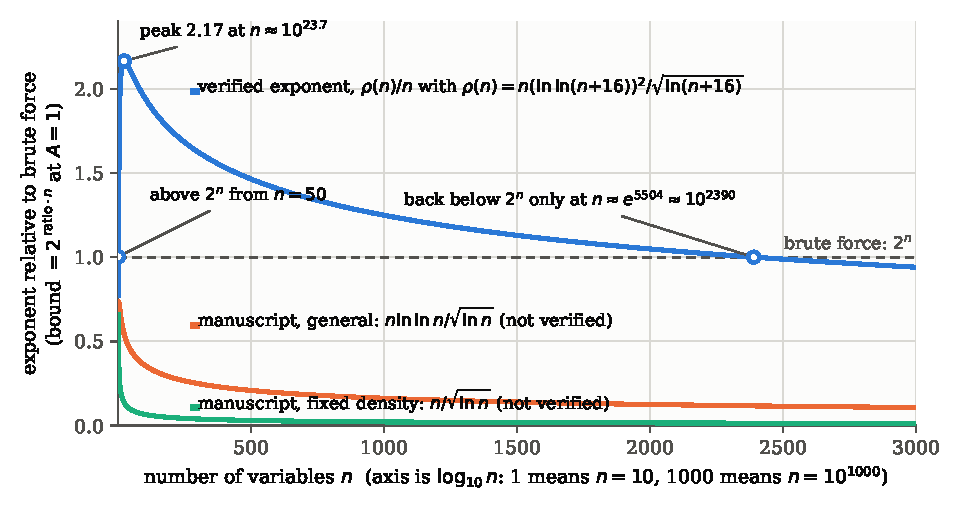
\includegraphics[width=\linewidth]{rho_over_n.pdf}\\[4pt]
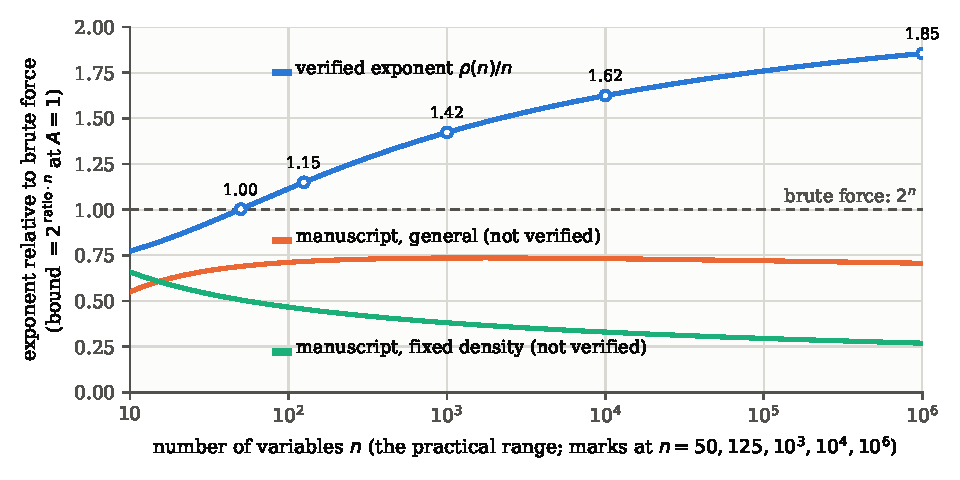
\includegraphics[width=\linewidth]{rho_over_n_practical.pdf}
\caption{The verified exponent against trying every assignment. Each
curve is an exponent divided by $n$; the dashed line at $1$ is $2^n$,
the cost of trying every assignment, and a curve above the line is a
guarantee worse than that. Top: the whole range, the horizontal axis
being the number of digits of $n$, from $n = 10$ to $n = 10^{3000}$.
The solid curve is the verified exponent $\rhon/n$; the two curves
beneath it are the manuscript's two sharper exponents,
$n\ln\ln n/\sqrt{\ln n}$ (the manuscript's Theorem~1.1, general case) and $n/\sqrt{\ln n}$ (its fixed-clause-density case), which are not in the Lean library
(Section~\ref{sec:beyond}). Bottom: the same three curves over the
practical range $n = 10$ to $10^6$, with $\rhon/n$ marked at $n = 50,
125, 10^3, 10^4, 10^6$. All curves take the constant $A$ to be $1$; the
verified $A$ is unknown and at least 257 in the proof on record.
Regenerate: \texttt{python3 -I paper3/scripts/rho\_over\_n.py}.}
\label{fig:central}
\end{figure}

\begin{figure}[htbp]
\centering
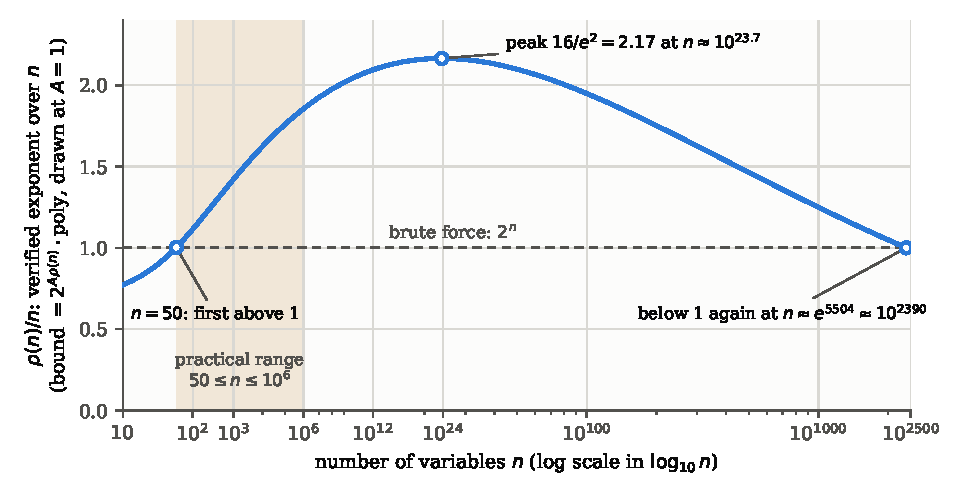
\includegraphics[width=\linewidth]{runtime_scale.pdf}
\caption{The ratio $\rhon/n$ alone, over an enormous range: the
horizontal axis is the number of digits of $n$, from $n = 10$ to
$n = 10^{2500}$. The level $1$ is the cost of trying every assignment.
Marked: the first whole number above the level ($n = 50$); the peak
($16/e^2 = 2.17$, at $n \approx 10^{23.7}$); the return below the level
($n \approx e^{5504} \approx 10^{2390}$); and, shaded, the practical
range $50 \le n \le 10^6$. Regenerate:
\texttt{python3 -I paper3/scripts/runtime\_scale.py}.}
\label{fig:runtime-scale}
\end{figure}

\subsection{The title's claim, made precise}
\label{sec:statement-title}

The title says the verified algorithm is slower than trying all $2^n$
assignments at every practical size. Read against the theorem, that
means the following four things, and nothing more.

\begin{enumerate}
\item \textbf{What is verified is a guarantee, not a running time.} The
  theorem says the machine halts within $C(L+1)^d\,2^{A\rhon}$ steps.
  It does not say how many steps the machine actually takes on any
  input. No implementation of the machine exists to be timed. A bound
  above $2^n$ does not say the machine is slow; it says the proof
  promises nothing better than $2^n$ there.
\item \textbf{The constants are never computed.} The theorem asserts
  that $C, A, S, d, e$ exist. The proof builds them from other
  existence lemmas and states no value, beyond the $A \ge 257$ read
  above. The machine's number of states is likewise never computed.
\item \textbf{With $A = 1$, the verified exponent is above $n$ for every
  $n$ from 50 up to about $10^{2390}$.} That is
  Table~\ref{tab:runtime-scale}. Over that range the exponential part
  of the bound is at least $2^n$, and at its worst it is $2^{2.17\,n}$.
  With the true $A$, whatever it is, the exponential part is $2^{A\rhon}$,
  which is at least $2^{\rhon}$ as soon as $A \ge 1$; and the proof's
  own construction has $A \ge 257$. So nothing on record puts the bound
  below $2^n$ at any practical size.
\item \textbf{Hence, at every practical size, the verified guarantee is
  weaker than the guarantee of trying all assignments.} Trying all
  $2^n$ assignments and checking each against the $m$ clauses counts
  the satisfying ones in $2^n$ times a small polynomial in $n + m$
  steps, with constants one can write down. The verified guarantee is
  $C(L+1)^d\,2^{A\rhon}$ with $\rhon > n$ on $50 \le n < e^{5504}$ and
  $C, A, d$ unknown. For every $C \ge 1$, $A \ge 1$ and $d \ge 1$ the
  verified bound is above $2^n$ on every $n$ in that range. The only
  values on record are the proof's own, which has $1 \le C$ and
  $1 \le A$ in the statement of its main run
  (\clonefile{SqrtLogSpace/NativeLargeEntry.lean}, line 12) and
  $A \ge 257$ in its construction. A proof with $A < 1$ would be a
  different proof; none is on record.
\end{enumerate}

None of this is a defect of the formalisation or of the proof. It is
what a theorem of this shape means when the constants in it are not
tracked. The manuscript itself calls $\rhon$ ``the weaker exponent''
(p.~2, line~63), and its sharper exponents are not in the Lean library
(Section~\ref{sec:beyond}). One detail of bookkeeping: inside the
solution the exponent is written with base-2 logarithms, and a lemma shows the two forms differ only by a fixed multiplier, which can be folded into the constant $A$ (Appendix~\ref{app:tech-theorem}); nothing above depends on it.

\subsection{What the statement does establish}
\label{sec:statement-establishes}

For each fixed width $k \ge 2$, there is a deterministic machine that,
given any $k$-CNF on $n$ variables with $m$ clauses in the fixed
encoding, halts with the exact number of satisfying assignments written
in binary on a named tape, within $C(L+1)^d\,2^{A\rhon}$ steps. Here
$L$ grows no faster than a polynomial in $n + m$, and $\rhon$ grows more
slowly than $n$. A formula of width $k$ on $n$ variables cannot have
more than about $n^k$ distinct clauses ($2{,}604{,}376$ at $n = 125$,
$k = 3$; Appendix~\ref{app:tech-theorem}), so the whole bound is
subexponential in $n$ alone. In the standard vocabulary, where $o(n)$ means a quantity that grows more slowly than $n$ and $\mathrm{poly}$ a polynomial: a deterministic $2^{o(n)} \cdot \mathrm{poly}(n+m)$ algorithm for counting the solutions
of $k$-SAT, and therefore for deciding it. That refutes the Exponential
Time Hypothesis \citep{ImpagliazzoPaturi2001}, the conjecture that
3-SAT needs time exponential in $n$, as stated. The verified theorem is
the manuscript's own verified form, the weaker exponent of its
Proposition~6.4 (p.~43, lines 2474--2476), without the $n \ge 20$
condition. We found no field, definition or quantifier through which
the statement could be accepted by the kernel and yet mean something
weaker than this; the audit behind that sentence is
\repofile{reports/scratch/eth_audit/statement_audit.md}. Our own
restatement of the theorem as a named Lean sentence, over a verbatim
copy of the machine model, is \leanref{subexpcount}; it is never proved
and never assumed there (Section~\ref{sec:lean}).

\subsection{What this does not claim}
\label{sec:statement-not}

\begin{itemize}
\item \textbf{No running time of any machine.} Nothing here measures or
  estimates how long the verified machine, or any program, takes on any
  input. The title compares two \emph{guarantees}.
  Section~\ref{sec:practitioner} is the only place in the paper where
  anything is timed, and it times ordinary solvers, not this machine.
\item \textbf{No statement about the proof.} That the statement means
  what we say it means is a reading of 220 lines. Whether the proof is
  sound is Section~\ref{sec:proof} and Section~\ref{sec:replay}, which
  found no flaw. The one proof-side fact quoted here, $A = 256 + A_t$,
  is a line of the solution read for the value it assigns, not a claim
  about the argument.
\item \textbf{No value of the constants.} $A \ge 257$ is what the proof
  writes down, not what the machine needs; a different proof of the
  same statement could have any $A > 0$. The statement itself fixes
  nothing.
\item \textbf{Nothing about the manuscript's sharper exponents}, which
  are not in the Lean library and are Section~\ref{sec:beyond}'s
  subject.
\item \textbf{No claim about sizes beyond $e^{5504}$.} Past
  $n \approx 10^{2390}$ the verified exponent is below $n$ again at
  $A = 1$; we say nothing about that range except that it is not a
  practical one.
\end{itemize}
\par\endgroup
